\documentclass[a4paper, 11pt]{article}
\usepackage{geometry}
\geometry{letterpaper, margin=1in}
\usepackage{amsmath}
\usepackage{amssymb}  
\usepackage{amsthm}
\usepackage{ulem} 
\usepackage{graphicx}
\usepackage{enumitem} % use for making lettered list 
\usepackage{bbm} % use for making the 1 identity operator EX: \mathbbm{1}
\usepackage{subfig} 
\graphicspath{ {images/} }

% format to allow bolded theorems, corollaries, etc... 
\newtheorem*{theorem}{Theorem}
\newtheorem*{corollary}{Corollary}
\newtheorem*{lemma}{Lemma}
\newtheorem*{definition}{Definition}

% stop typing \mathbb a thousand times 
\newcommand{\R}{\mathbb{R}}
\newcommand{\C}{\mathbb{C}}



\begin{document}
%Header-Make sure you update this information!!!!
\noindent
\large\textbf{Abstract Surfaces} \hfill \textbf{John Waczak} \\
\normalsize MTH 435 \hfill  Date: \today \\
Dr. Christine Escher \\
\par\noindent\rule{\textwidth}{0.4pt}	
	
\subsection*{Problem 1}
	\textit{Introduce a metric on the projective plane $\mathbb{R}P^2$ so that the natural projection $\pi:S^2\to\mathbb{R}P^2$ is a local isometry. What is the Gaussian curvature of such a metric?}

	\begin{proof}
		Recall that the natural projection $\pi:S^2\to\mathbb{R}P^2$ is defined such that $\forall p \in S^2$, $\pi(p) = [p] = \{p, A(p)\}$ where $A:S^2\to S^2$ is the antipodal map. We want to choose a metric $\langle , \rangle$ for $\mathbb{R}P^2$ such that $\pi$ is a local isometry. This means that for $p\in S^2$ and $\forall x,y \in T_p S^2$ we need 	
			\begin{equation*}
				\big\langle x,y \big\rangle_p = \big\langle d\pi(x), d\pi(y) \big\rangle_{\pi(p)}
			\end{equation*}
		
		\noindent Recall that $d\pi:T_p S^2 \to T_{\pi(p)}\mathbb{R}P^2$ is a linear transformation. We also showed in class that specific charts $X_i:U\subset \mathbb{R}^2 \to S^2$ induce an associated basis on the tangent space. Thus, let $p\in S^2$ such that $p= X_i(u,v)$ for some $u,v \in U$ and let $q\in \mathbb{R}P^2$ such that $q=\pi(p)$. Then $\forall a,b \in T_{\pi(p)}\mathbb{R}P^2$ and $\alpha,\beta,\gamma,\delta\in\mathbb{R}$, we can write 
			\begin{align*}
				a &= \alpha\Big(\pi \circ X_i(u,v)\Big)_u + \beta\Big(\pi \circ X_i(u,v)\Big)_v \\ 
				b &= \gamma\Big(\pi \circ X_i(u,v)\Big)_u + \delta\Big(\pi \circ X_i(u,v)\Big)_v 
			\end{align*} 
		\noindent Where I have written $\pi(p)_u, \pi(p)_v$ to denote the associated basis for the tangent space. Now define $a',b'\in T_{p=X_i(u,v)}S^2$ such that 
			\begin{align*}
				a' &= \alpha \Big(X_i(u,v)\Big)_u + \beta \Big(X_i(u,v)\Big)_v \\ 
				b' &= \gamma \Big(X_i(u,v)\Big)_u + \delta \Big(X_i(u,v)\Big)_v 
			\end{align*}
		\noindent Where $a',b'$ are the points in the tangent space associated with the scaling factors $\{\alpha,\beta,\gamma\delta\}$. From the linearity of $d\pi$ we can write
			\begin{align*}
				d\pi(a') &= d\pi \Big[ \alpha \Big(X_i(u,v)\Big)_u + \beta \Big(X_i(u,v)\Big)_v  \Big] \\ 
					&= \alpha d\pi\Big(X_i(u,v)\Big)_u + \beta d\pi\Big(X_i(u,v)\Big)_v \\ 
					&= \alpha\Big(\pi \circ X_i(u,v)\Big)_u + \beta\Big(\pi \circ X_i(u,v)\Big)_v = a 
			\end{align*}
		So $d\pi(a') = a$ and repeating this process for $b'$ gives $d\pi(b') = b$. Therefore, to induce an isometry, choose a metric $\langle , \rangle$ such that 
			\begin{equation*}
				\langle a, b \rangle_{\pi(p)} \equiv \langle a', b' \rangle_p 
			\end{equation*}
		Then $\forall x,y \in T_p S^2$ we have that 
			\begin{equation*}
				\big\langle x, y \big\rangle_p = \big\langle d\pi(x), d\pi(y)\big\rangle_{\pi(p)}  
			\end{equation*}
		Because our choice of metric on $\mathbb{R}P^2$ induces a local isometry with $S^2$ then the Gaussian curvature of $S^2$ is preserved by the isometry $\pi$. Thus the curvature of $\mathbb{R}P^2$ under our metric must be 1. 
	\end{proof}

\subsection*{Problem 2 (The Infinite Mobius Strip)} 
	\textit{
		Let $C=\{(x,y,z)\in \R^3 : x^2+y^2 = 1\}$ be a cylinder and $A:C\to C$ be the map (antipodal map) such that $A(x,y,z) = (-x,-y,-z)$. Let $M$ be the quotient of C by the equivalence relation $p\sim A(p)$ and let $\pi:C\to M$ be the map $\pi(p) = [p] = \{p, A(p)\}$, $p\in C$. 
		\begin{enumerate}[label=(\alph*)]
			\item Show that $M$ can be given a differentiable structure so that $\pi$ is a local diffeomorphism ($M$ is then called the infinite Mobius Strip) 			
			\item Prove that M is non-orientable 			
			\item Introduce a Riemannian metric on M so that $\pi$ is a local isometry. What is the curvature of such a metric. 
		\end{enumerate}
		}

		\begin{proof}[(a)]
			Recall that a \textbf{differentiable structure} is the family of open subsets of $\R^2$ denoted $U_\alpha$ together with coordinate charts on those open subsets that take $U_\alpha \to S$. These charts are denoted $X_\alpha$ and are referred to collectively as $\{U_\alpha, X_\alpha\}$. \\
			
			\noindent We need to show that $M$ can be given a differentiable structure $(U_\alpha, \pi\circ X_\alpha)$ so that $\pi$ is a local diffeomorphism. To be a local diffeomorphism we need the image $\pi\circ X_\alpha(U_\alpha)$ to be open in $M$ for all $\alpha$ and that $\pi\circ X_\alpha$ is a smooth bijection with smooth inverse. First, it is clear that the antipodal map $A(p)$ is a diffeomorphism. The only operation is multiplying each coordinate by the scalar (-1) which is smooth. It's inverse also looks pretty much exactly the same. Therefore, to make $\pi$ a diffeo we need to choose $U_\alpha$ so that we have this diffeomorphism. The problem with $\pi$ is that if $\mathbf{x}_\alpha(U_\alpha)\cap A\circ\mathbf{x}_\alpha(U_\alpha)\neq \emptyset$ we do not have an injective function as two points (i.e. $p, A(p)$) both get sent to $[p]$. $\pi$ is certainly surjective as every point in $\pi\circ\mathbf{x}_\alpha(U_\alpha)$ has a point in the preimage $\mathbf{x}_\alpha(U_\alpha)$. Therefore if we choose our $U_\alpha$ so that $\mathbf{x}_\alpha(U_\alpha)\cap A\circ\mathbf{x}_\alpha(U_\alpha) = \emptyset$ then $\pi$ will be a diffeomorphism. 			
 
		\end{proof}

		\begin{proof}[(b)]
			First I will try and prove a small lemma stating that if an open subset of an abstract surface $S$ is diffeomorphic to the open mobius band, then $S$ is nonorientable. Recall that the standard Mobius band is nonorientable. We showed this previously (Tapp Proposition 3.54) by showing that any unit normal field $N$ on the strip would have two possible directions for a given point $p$. This definition must be equivalent to the abstract surface definition for orientable given in this assignment (NOTE: I couldn't figure out how to use the new definition to show that the finite mobius band is nonorientable)\\
			
			\noindent Then all that remains is to show that any open subset M of an abstract surface S is nonorientable if it is diffeomorphic to the mobius band. Define $M_b$ to be the finite mobius band. Assume for contradiction that $S$ a regular surface, is orientable. Then there must exists a family of parametrizations covering $S$ such that all coordinate changes have a positive Jacobian. Restriction of this family to the open subset $M\subset S$ that is diffeomorphic to $M_b$ must induce an orientation on M. This is a contradiction though because $M_b$ is diffeomorphic to $M$ and therefore nonorientable. \\ 
			
			\noindent Armed with this fact, we simply need to identify a finite mobius band contained within a subset of our abstract surface M created by considering the quotient space of the cylinder $C$ by the equivalence relation $p\sim A(p)$. Do Carmo was able to identify such a band in the real projective plane (page 436) as shown in the following diagram:  \\ 
			\pagebreak 
				\begin{figure}[!hbt]
					\centering
					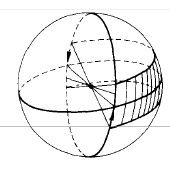
\includegraphics[width=0.25\columnwidth]{mobiusStrip_realProjective}
				\end{figure}
		
			\noindent Where the Mobius strip is identified along the equator. Following a similar construction, we can identify a finite mobius band on our $M$ as shown in the following illustration. 
				\begin{figure}[!hbt]
					\centering
					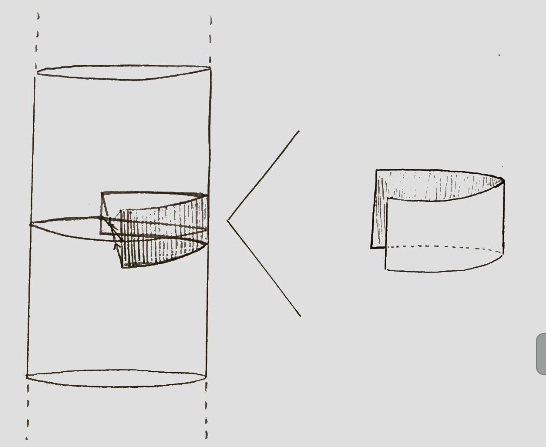
\includegraphics[width=0.45\columnwidth]{mobiusBand_cylinderAntipodal}
				\end{figure}
			Therefore because we have identified a mobius strip within a subset of our surface, $M$ is nonorientable. 
		\end{proof}

		\begin{proof}[(c)]
			To introduce a Riemannian metric on M that makes $\pi$ a local isometry, we can repeat the same procedure as in problem one. Choose a Riemannian metric $\langle , \rangle$ such that $\forall a,b \in T_{\pi \circ \mathbf{x}_\alpha(u,v)}M$ 
			such that 
				\begin{align*}
					a &= \alpha(\pi\circ\mathbf{x}_\alpha(u,v))_u + \beta(\pi\circ\mathbf{x}_\alpha(u,v))_v \\ 
					b &= \delta(\pi\circ\mathbf{x}_\alpha(u,v))_u + \gamma(\pi\circ\mathbf{x}_\alpha(u,v))_v
				\end{align*}
			and $a',b' \in T_{\mathbf{x}_\alpha(u,v)}C$ 
				\begin{align*}
					a' &= \alpha(\mathbf{x}_\alpha(u,v))_u + \beta(\mathbf{x}_\alpha(u,v))_v \\ 
					b' &= \delta(\mathbf{x}_\alpha(u,v))_u + \gamma(\mathbf{x}_\alpha(u,v))_v
				\end{align*}
			we have 
				\begin{equation*}
					\langle a, b \rangle = \langle a', b' \rangle 
				\end{equation*}
			Then $\pi$ will be an isometry as we saw in problem 1. If $\pi$ is an isometry, it must preserve the Gaussian curvature. Therefore the curvature of $M$ under such a metric will be the same as that of the cylinder: 0. 
		\end{proof}

\subsection*{Problem 3}
	\textit{\begin{enumerate}[label=(\alph*)]
			\item Show that the projection $\pi:S^2\to\R P^2$ from the sphere onto the projective plane has the following properties. (1) $\pi$ is continuous and $\pi(S^2) = \R P^2$. (2) each point $p\in \R P^2$ has a neighborhood U such that $\pi^{-1}(U) = V_1 \cup V_2$ where $V_1$ and $V_2$ are disjoint upen subsets of $S^2$ and the restriction of $\pi$ to each $V_i, \quad i=1,2$ is a homeomorphism onto U. Thus $\pi$ satisfies formally the conditions for a covering map with two sheets. Beacaus of this, we say that $S^2$ is an orientable double covering of $\R P^2$.  	
			\item Show that in this sense, the torus $T$ is an orientable double covering of the Klein bottle $K$ and that the cylinder is an orientable double covering of the infinite Mobius strip. 
		\end{enumerate}}
		
	\begin{proof}[(a)]
		We can show that $\pi$ is continuous by showing that the inverse image of every open set is an open set, i.e. that $\pi^{-1}(V)$ is open in $S^2$ for some open set $V$. This is true as we chose our $U_\alpha$ to be open subsets of $\R^2$ such that $\bigcup_\alpha \mathbf{x}_\alpha(U_\alpha) = S^2$. Thus any open set $V$ has a preimage that lies in an open set $\mathbf{x}_\alpha(U_\alpha)$ or in the intersection of two (or more) open sets $\mathbf{x}_\alpha(U_\alpha)\cap\mathbf{x}_\beta(U_\beta)$ which is an open set. $\pi(S^2) = \R P^2$ by construction (this is how we defined $\R P^2$ in class).\\ 
		
		
		 \noindent Recall that we defined our open sets $U_\alpha$ so that $\mathbf{x}_\alpha(U_\alpha)\cap A\circ\mathbf{x}_\alpha(U_\alpha) = \emptyset$. This means that so long as we take our neighborhood of $p\in \R P^2$ to be given by $\pi\circ\mathbf{x}_\alpha(U_\alpha)$ for such a $U_\alpha$ then the preimage $\pi^{-1}(p)$ is in the disjoint union $\mathbf{x}_\alpha(U_\alpha)\cup A\circ\mathbf{x}_\alpha(U_\alpha)$ on the sphere. The restriction of $\pi$ to one such $\mathbf{x}_\alpha(U_\alpha)$ is a homeomorphism because the antipodal map $A(p)$ is a diffeomorphism. Therefore $S^2$ is the orientable double covering of $\R P^2$. 
	\end{proof} 
	
	\begin{proof}[(b)]
		In this same vein, it follows that the torus $T$ and the cylinder $C$ are orientable double coverings of the Klein bottle $K$ and the infinite mobius strip because we used the same mapping $\pi$ which maps points in each surface to their equivalence class by the antipodal map i.e. $p\mapsto [p] = \{p, A(p)\}$. All of the same parts of (a) still apply. 	
	\end{proof}

\subsection*{Problem 4} 
	\textit{Extend the Gauss-Bonnet theorem to orientable Riemannian 2-manifolds and apply it to prove the following fact: There is no Riemannian metric on an abstract surface $T$ diffeomorphic to a torus such that its curvature is positive (or negative) at all points of T }

	Recall that the Global Gauss-Bonnet Theorem stated:
		\begin{definition}
			If S is an compact, regular surface, then	
				\begin{equation*}
					\iint_S KdA = 2\pi\chi(S)
				\end{equation*}
		\end{definition}
		
	\noindent We want to extend this definition to surfaces. Certainly, all of our notions of curves in surfaces exists as our curves are just differentiable functions $\alpha:(-\varepsilon, \varepsilon) \to S $. Furthermore, our notion of Gaussian curvature makes sense as all we showed previously that this is an intrinsic quantity that only depends on our $E, F, G$ functions (now given by our choice of Riemannian metric). Lastly, because we know that any compact, regular surface can be triangulated, we can triangulate on our compact, abstract surfaces. Because triangulation makes sense, we can define the Euler Characteristic. The last thing I think we need to justify is the idea of integration. This still makes sense when we consider that the integral can be rewritten as $\iint_{\mathbf{x}_\alpha^{-1}}K||d\mathbf{x}_\alpha||dA$. Then $dA = dudv$ (the regular old surface element) and $||d\mathbf{x}_\alpha||$ is the area distortion. $d\mathbf{x}_\alpha$ is well defined as the linear transformation from $\R^2 \to T_{\mathbf{x}_\alpha(u,v)}S$. \\ 
	
	\noindent Now that we have all of the tools, consider an abstract surface $T$ that is diffeomorphic to the Torus. Assume for contradiction that this surface has strictly positive or strictly negative curvature. Then because this surface is diffeomorphic to the Torus which is compact, we can apply the Gauss-Bonnet to show
		\begin{equation}
			\iint_T K dA = 2\pi\chi(T)
		\end{equation}
	\noindent Now because this abstract surface is diffeomorphic to the Torus it's Euler Characteristic must be $\chi(T) = \chi(\text{torus}) = 0$ Therefore
		\begin{equation*}
			\iint_T K dA = 2\pi(0) = 0 
		\end{equation*}

	\noindent Clearly then, if K is strictly greater than zero we have a contradiction as the sum of positive values can not evaluate to zero. The same is true for the second case because summing strictly negative numbers can not return 0. Therefore it must follow that there is no abstract surface diffeomorphic to the torus with strictly positive or negative Gaussian curvature. Now, the Gaussian Curvature can be intrinsicly defined solely in terms of our $E, F, G$ functions i.e. the Riemannian metric. Thus because we are not allowed to have a entirely positive or negative curvature on an abstract surface diffeo to the torus, there is no way to E, F, and G functions to can force this to work and so there must be no Riemannian metric satisfying this condition. 




		
		
\end{document}




































